\documentclass[../Cryptography.tex]{subfiles}

\begin{document}
\chapter{Secret-key techniques}
We now study the case of symmetric crypto. In symmetric crypto, Ali and Bachar have one key each, and this key is private. This is very important to hold into account. In asymmetric crypto, each one has a public key, a private key, must know the public key of his collegues, etc. But here, none of that : an encryption scheme works under a private key. This is why this is the simplest case to study and the first one we study. \\

We are thus interested here in building a secure encryption scheme, that gets as input a message in plaintext and outputs a ciphertext, as well as a decryption algorithm that allows us to retrieve the message. The definitions of IND-CPA was made very clear : if the system is secure, an adversary that does not know the key has better chance of going random instead of trying to guess ! \\

There are many functions needed to build to \textit{in fine} build a secure symmetric encryption scheme. There is the mechanism of the key, and some more functions such as block ciphers, permutations, etc. All these are useless separately, but at the end they build an encryption scheme. In this course, we will cover :
\begin{itemize}
    \item Keystream generators and stream ciphers
    \item Block ciphers
    \item Permutations
\end{itemize}

\section{Basic schema}
The basic schema of the communication is the following : Ali wants to send a message to Bachar. Then :
\begin{itemize}
    \item \underline{One key} is generated and given to Ali, and to Bachar, under a \textbf{secure channel}.
    \item Ali encrypts the message with the key $k$,
    \item transmits it to Bachar in a public channel, in clear : any outsider Omar\footnote{Instead of Oscar.} can observe the thing sent.
    \item Bachar receives the ciphertext, and decrypts it with the same key $k$.
\end{itemize}

\section{Stream ciphers vs block ciphers}
There are two ways of doing symmetric crypto : with stream ciphers of with block ciphers. \\

\begin{itemize}
    \item Stream ciphers process a message bit by bit, XORing every bit with a key stream $s_i$ built from the original key by a keystream generator.
    \item Block ciphers process a message by separating it into blocks, and processing block by block. Within a block, each bit value has an impact on the output for the block.
\end{itemize}

\section{Keystream generators and stream ciphers}
Stream ciphers are simple : they need a key as long as the plain text and they XOR it with the message. For this, we take a private key $k$ that is not necessarly very long, and we extend it, building a key stream $s = (s_i)$. This key stream generation process is the main focus for stream ciphers. \\

The encryption and decryption algorithm are as follows, with the generated key stream $s=(s_i)$. We notice that the two algorithms are the same. It indeed works.

\begin{center}
    \includegraphics[width=0.8\linewidth, page = 7]{Slides/2-Secret.pdf}
\end{center}


\section{Block ciphers}
A block cipher is basically a mapping from :
\begin{itemize}
    \item Input : secret key $k\in \mathbb{Z}_2 ^m$, and \textbf{input block} $x \in \mathbb{Z}_2 ^n$
    \item Output block $y = E_k(x) \in \mathbb{Z}_2 ^n$.
\end{itemize}
And we ensure that for each key $k$, the function has an inverse : $x = E_k ^{-1}(y)$. \\

Note that as it is, we can not use it as encryption scheme, it is completely deterministic so it loses the IND-CPA game. \\



\subsection{DES}
DES is a block cipher : it takes a block as input, a key, and generates an output block. For a classical DES algorithm, the input block has 64 bits and the key is 56-bits long. Actually, 64 bits come as input for the key, but every 7\textit{th} bit is used as a parity bit, not a key bit. DES is a 56-bit cipher. \\

$$x \in \mathbb{Z}_2 ^{64} \qquad k \in \mathbb{Z}_2 ^{56}$$

With the input block $x$ and the key $k$, DES works by computing 16 rounds of its underlying network. For each round, it needs a key, that is derived from the original key. Those are subkeys $K_i$.

$$k \Rightarrow K_1, K_2, \dots K_{16} \in \mathbb{Z}_2 ^{48}$$
The section below explains how the subkeys (also called \textit{round keys} are generated).
\subsubsection{Key schedule : round keys generation}
Input : the 56-bits key. It is all based on permutations, and more precisely on two permutations : PC-1 and PC-2. Here is how 16 48-bits keys are generated.
\begin{enumerate}
    \item The initial key goes under a bit transposition, through the table of permutation of PC-1 (see figure below). So at the exit of PC-1, we still have a 56-bit key. We separate it into two 28-bits blocks : $C_0$ and $D_0$.
    $$\mathrm{PC}1 \; : \; \mathbb{Z}_2 ^{56} \rightarrow \mathbb{Z}_2 ^{56}$$
    
    \item For $i$ going from 1 to 16 :
        \begin{itemize}
            \item We build $C_i$ from $C_{i-1}$, $D_i$ from $D_{i-1}$, thanks to a permutation $LS_i$
            \item $LS_i$ is a circular shift to the left : by one when $i=1, 2, 9, 16$, by two positions otherwise
            \item $K_i$ is obtained by the concatenation $C_i \Vert D_i$ but again under a permutation. This time, it is PC-2 that handles it, and ignore some bits to make it fit in 48 bits : 
            $$\mathrm{PC}2 \; : \; \mathbb{Z}_2 ^{56} \rightarrow \mathbb{Z}_2 ^{48}$$
        \end{itemize}
\end{enumerate}
\begin{center}
    \includegraphics[width=0.5\linewidth, page=23]{Slides/2-Secret.pdf}
\end{center}

\subsubsection{DES's $f$ function}
At each round, the current state is processed, divided into two blocks, $L_{i-1}$ and $R_{i-1}$, using $K_{i}$ and a function called $f$. DES's $f$ function works as follows : it takes a 32-bit input, which is the half-message block, and the subkey.

$$f : \mathbb{Z}_2 ^{32} \times \mathbb{Z}_2 ^{48} \rightarrow \mathbb{Z}_2 ^{32}$$
\begin{center}
    \includegraphics[height=7cm]{images/2-DES-feistel.png}
    \includegraphics[page=19, height=7cm]{Slides/2-Secret.pdf}
\end{center}
The $S-$boxes are what make DES non linear, crucial for cryptanalysis.

\subsubsection{Non-ideal properties}
\begin{itemize}
    \item There are some weak keys (4) for which DES is an involution
    \item There are some weak pairs (6) of keys for which DES is an involution 
    \item Complementarity property : $ E_k(x) = y \iff E_{\bar{k}}(\bar x) = \bar y$ reduces the Exhaustive search by 2 (one bit).
\end{itemize}
\subsubsection{Flaws of DES}
\begin{itemize}
    \item Size of the key space : 56 bits is very small... Exhaustive search can be done in $2^{55}$ operations, which is nowadays feasible.
    \item Susceptible to mathematic cryptanalysis : differential, linear. 
\end{itemize}

\subsubsection{Triple-DES}
An improvement is then to take larger keys, for example three keys and building Triple-DES with 168 bits ($= 3\times 56$), with two keys, 112 bits. Note that 3DES is retro-compatible with single DES, we just have to huse thrice the same key.
$$3\mathrm{DES}_{k_1\Vert k_2\Vert k_3} = \mathrm{DES}_{k_3} \circ \mathrm{DES}_{k_2} ^{-1} \circ \mathrm{DES}_{k_1} $$
$$3\mathrm{DES}_{k_1\Vert k_2} = \mathrm{DES}_{k_1} \circ \mathrm{DES}_{k_2} ^{-1} \circ \mathrm{DES}_{k_1} $$

Why not simple Double-DES ? Because with two rounds of DES, one can make two times a brute force, one for each system, and breaking the system, in a time of $2^{57}$ and using memory $2^{56}$ : storing every attempt on the first system (intercepting information before it comes to the second DES layer), then trying to decrypt the second DES with the saved attempts.

\subsection{Rijndael and AES}
With such flaws for DES, it stinks. Rijndael comes to help. We talk of Rijndael as AES, you should know it, and if you don't, Google the origins. Anyway, AES takes as input a 128-bits block, and there are multiple cases for the key, and for each case ther is a number of rounds of the cipher :
\begin{itemize}
    \item AES-128 : 128-bits key : 10 rounds
    \item AES-192 : 192-bits key : 12 rounds
    \item AES-256 : 256-bits key : 14 rounds
\end{itemize}
\subsubsection{Representation of $x$ in the Galois Field}
$x$ is represented as a $4\times 4$ array in the Galoid Field. It is called at any point the \textbf{state} of the algorithm. The key, $k\in \mathbb{Z}_2 ^{128}$. \\

\subsubsection{Round of AES}
It works by \textbf{layers}. Each round contains 3 layers :
\begin{itemize}
    \item Key addition layer : a 128-bit round key, or subkey, which has been derived from the main key in the key schedule, is XORed to the state
    \item Byte Substitution layer (S-Box) Each element of the state is nonlinearly transformed using lookup tables with special mathematical properties. This introduces \textit{confusion} to the data, i.e., it assures that changes in individual state bits propagate
    quickly across the data path.
    \item Diffusion layer : it consists of two sublayers,
both of which perform linear operations, in order to provide diffusion over all state bits :
    \begin{enumerate}
        \item \textit{ShiftRows} : permute the data on a \textbf{byte} level
        \item \textit{MixColumns} : matrix multiplication which combines, mixes, blocks of 4 bytes ($s_1, ..., s_4$). Here, if one of the values change, the hole state changes.
    \end{enumerate}
\end{itemize}

\begin{center}
    \includegraphics[width=0.8\linewidth, page=43]{Slides/2-Secret.pdf} \\
    \includegraphics[page=45, width=0.45\linewidth]{Slides/2-Secret.pdf}
    \includegraphics[page=47, width=0.45\linewidth]{Slides/2-Secret.pdf} \\
    \includegraphics[page=48, width=0.45\linewidth]{Slides/2-Secret.pdf}
    \includegraphics[page=51, width=0.45\linewidth]{Slides/2-Secret.pdf}
\end{center}
\subsubsection{Quick chat about Galois Field}
In AES the finite field contains 256 elements and is denoted as $GF(2^8)$. This field is chosen because then each element of the field can be represented, in binary, by one byte. This is why in the S-box and MixColumns transforms, AES treats every byte of the internal data path as an element of the field $GF(2^8)$ and manipulates is by performing arithmetics in this finite field.
\subsubsection{Inverting AES}
As AES is not based on a Feistel network, all layers must be inverted for decryption. We begin by inverting last round, round $n_r$, then $n_{r-1}$ until round $1$.
\begin{itemize}
    \item We first go through the same key expansion algorithm to get the subkeys $K_i '$ from $k$ if needed (remember, we are dealing with symmetric crypto, encryption and decryption are with the same key!)
    \item With the ciphertext $y$ as input, we compute XOR with the last key chunk $K_{10, 12\text{ or} 14}$.
    \item Then, for each round, we compute the inverse of each step.
    \begin{itemize}
        \item SubBytes becomes InvSubBytes
        \item InvShiftRows
        \item InvMixColumns
        \item AddRoundKey stays the same (XOR)
    \end{itemize}
\end{itemize}
\subsection{Modes of operation}
Okay we've seen the famous block ciphers DES, AES, but what to do with them ? As we have already said, it can not constitute an encryption scheme that is IND-CPA, because of their deterministic kind. We must build another architecture using those. \\

\subsubsection{Electronic codebook (ECB)}
A first example of architecture using block ciphers is the \textbf{electronic codebook} (ECB). It takes as input a message $p$, a secret key, and a number $n$ which corresponds to the desired block length. So, $p$ is first padded to reach a length that is a multiple of the block size $n$, and then each block is processed the same way using the block cipher encryption with the key. It is represented at the left figure below. \\
$$c_i = E_k(p_i)$$
The problem here is of course that every similar block of plaintext is encoded the same way.

\subsubsection{Ciphertext block chaining (CBC)}
We take the same scheme as the ECB but at each round, the plaintext block is XORed with a vector before output. The first vector is an initialization vector (IV), and the vector to XOR with $p_i$ is $c_{i-1}$, nothing but the ciphertext of previous encryption. Note that we here also add \textbf{diversification} : the initialization vector is \textbf{random}, and it must be a \textbf{nonce}. Then :
$$\begin{array}{ll}
    c_0 &= E_k(p_0 \oplus \mathrm{IV}) \\
    c_i &= E_k(p_i \oplus p_{i-1}) \\
\end{array}$$
And to decrypt : 
$$p_i = E_k ^{-1}(c_i) \oplus c_{i-1}$$

\begin{center}
    \includegraphics[width=0.45\linewidth]{images/2-EBC.png}
    \includegraphics[width=0.45\linewidth]{images/2-CBC.png}
\end{center}
\subsubsection{Limits of CBC}
What are the limits of the CBC ? Here, we present the probability that for encryption with a same key, $c_i = c_j '$ for different ciphertext blocks.
\begin{align*}
    c_i &= c_j ' \\
    E_k(p_i \oplus c_{i-1}) &= E_k(p_j ' \oplus c_{j-1}') && \text{By def.} \\
    p_i \oplus c_{i-1} &= p_j \oplus c_{j-1}' && \text{Because $E$ invertible} \\
    p_i \oplus p_j ' &= c_{i-1} \oplus c_{j-1}'
\end{align*}
Then, like we saw for the OTP, this means information is revealed on the plaintext ! But how likely is it that $c_i = c_j'$ ? This is related to the birthday paradox. Indeed, here, the ciphertexts of different blocks and different encryptions (same key, but other diversifier) are supposed to be completely random in respect with each other. Then, the probability of having such a \textit{collision} is left to randomness. This is why it is related to the birthday paradox.

\bg{Birthday paradox}{
    With a block size of $n$, the probability to get a collision after $L$ attempts is $$\mathrm{Pr}[\mathrm{coll.}] = \dfrac{L^2}{2^{n+1}}$$ which means that it tends to $1/2$ if $$L \sim 2^{n/2}$$.
}
\begin{itemize}
    \item For DES, the block size is 64 ($n=64$), so the number of blocks resulting from the message must be of $2^{32}$ in order to have a problem. This is a large number, but not really.
    \item For AES, the block size is 128, which gives us $2^{64}$ blocks before having a big probability of collision.
\end{itemize}
The birthday paradox is hence more a problem for DES.
\subsection{Counter mode}
The Counter mode (CTR) is also an encryption mode that uses block cipher as stream cipher.
\begin{itemize}
    \item Inputs : 
    \begin{itemize}[label = $\cdot$]
        \item Secret key $k \in \mathbb{Z}_2 ^m$
        \item Plaintext $p \in \mathbb{Z}_2 ^*$
        \item Diversifier $d \in \mathbb{N}$
    \end{itemize}
    \item First, we put a target, the desired block size : $n$.
    \item Then, we cut our message $p \longrightarrow (p_1, p_2, \dots, p_x)$. Each block is of $n$ bits, except $p_x$ that does not even require padding.
    \item We can now begin. The key stream is computed as followed, for $i$ going from $1$ to $x$ :
    $$k_i = E_k(d\Vert i)$$
    The last key chunk, $p_x$ is truncated to the length of $p_x$
    \item Encryption of block $i$ :
    $$c_i = k_i  \oplus p_i$$
    \item Output : $c \in \mathbb{Z}_2 ^*$
\end{itemize}
To decrypt, we can use the \textbf{same keystream} (remember that the nonce is public!) :
$$p_i = k_i \oplus c_i$$

\subsection{Build MAC from block cipher : CBC-MAC}
Aaaah, a bit of authentication ! Yes, block ciphers can also build MACs. Using the CBC architecture, but changing our goals, we can have :
\begin{itemize}
    \item Inputs :
    \begin{itemize}
        \item Secret key $k \in \mathbb{Z}_2 ^m$
        \item Message $m \in \mathbb{Z}_2 ^*$
    \end{itemize}
    \item Prepend $m$ with its length : $m \Rightarrow |m| \; \Vert m$
    \item Pad this with 1 and 0s, cut into blocks $(m_1, m_2, \dots, m_x)$
    \item Define $z_0 = 0 ^n$ and compute
    $$z_i = E_k(m_i \oplus z_{i-1})$$
    \item Output : MAC is $z_x$, the last chunk.
\end{itemize}
As we can see, we only keep the \textbf{last chunk} as output, in contrary with classical CBC. Verification goes by doing the same operation at home, with our key $k$ which is the same because of symmetric crypto, and see if we get the same MAC.

\subsection{Authenticated encryption}
As already said, we've seen primitives. Then we can combine them to create a scheme that is secure and provides authentication ! For example, we can encrypt with one key, and compute a MAC with another key (using CBC-MAC for example). Or there are also some modes that provide encryption and authentication with the same key.


\section{Permutations}
Permutations are also primitives, and they are very important. A \textbf{permutation is basically} a bijective mapping in $\mathbb{Z}_2 ^b$ :
$$f : \mathbb{Z}_2 ^b \rightarrow \mathbb{Z}_2 ^b$$A
As it is injective, is has an inverse. 

\subsection{The sponge construction}
With the help of permutations, we can build the following architecture, that is called a \textbf{sponge function}. \\

Two parameters, they are natural numbers : 
\begin{itemize}
    \item $r$ : bits of rate 
    \item $c$ : bits of capacity (security parameter)
\end{itemize}
and of course the permutation $f$. Together, they form a \textbf{sponge function} :
\begin{center}
    \includegraphics[width=0.6\linewidth, page=78]{Slides/2-Secret.pdf}
\end{center}
The output can be of any length that we want, we just need to add more rounds of $f$, this is why we see the $\infty$ symbol. \\

A keyed-sponge structure can be obtained if the message $m$ is prefixed with the secret key $K$.

\subsubsection{Keyed sponge for authentication}
Again, here, the goal is not to encrypt the text, but to build a MAC from the key and the message. When Bachar receives the message with the MAC, he has the secret key and can thus compute the same operation at home to verify that no Omar intercepted the message and changed it authenticity.
\begin{center}
    \includegraphics[width=0.5\linewidth, page=80]{Slides/2-Secret.pdf}
\end{center}
\subsubsection{Keyed sponge as a stream cipher}
Used here to build an encryption scheme : the sponge function acts as a key stream generator, and the encryption goes as it always do for stream ciphers.
\begin{center}
    \includegraphics[width=0.5\linewidth, page=81]{Slides/2-Secret.pdf}
\end{center}
\subsubsection{Authenticated encryption : spongeWrap}
Ewa c'est quoi la prochaine étape, spongeBob ?
\begin{center}
    \includegraphics[width=0.5\linewidth, page=82]{Slides/2-Secret.pdf}
\end{center}

\subsection{The duplex construction}
\includepdf[pages={2}]{Slides/Duplex.pdf}

\section{Pseudo-random functions}
\end{document}